\documentclass[11pt]{article}
\usepackage{../../styles/activity}

\usepackage{xr}
\externaldocument{0-MR}

\lhead{}
%\chead{\textbf{\Large{\hspace{0pt}Beginning Activities for Section~5.2}}\\\hspace{0pt}\emph{Mathematical Reasoning: Writing and Proof}}
\bahead{5.2}
\rhead{}
\lfoot{}
\rfoot{}
\cfoot{\hspace{0pt}\scalebox{0.4}{
\includegraphics{cc-by-nc-sa.eps}}}

\begin{document}
\input table

\subsection*{Beginning Activity 1 (Working with Two Specific Sets)}
In this beginning activity, we have our first example of proving one set is a subset of another set.  Proving subset relationships is a frequent type of proof when studying sets, and one of the usual methods of doing so is the \textbf{choose-an-element method}.  To prove a set $A$ is a subset of a set $B$, he idea is to choose an arbitrary element of $A$ and then use the definitions and properties of the two sets to prove that this element must also be an element of the set $B$.
\begin{enumerate} \setcounter{enumi}{1}
\item $S = \left\{ { \ldots ,  - 18,  - 12,  - 6, 0, 6, 12, 18,  \ldots } \right\}$ \quad
	$T = \left\{ { \ldots ,  - 6,  - 4,  - 2, 0, 2, 4, 6,  \ldots } \right\}$

It appears that  $S$  is a subset  of  $T$.

\item $S = \left\{ {x \in \mathbb{Z}\left. \right| x\text{ is a multiple of  6}} \right\}$ \quad
	$T = \left\{ {x \in \mathbb{Z}\left. \right| x\text{ is even}} \right\}$


\item An integer  $x$  is a multiple of  6  provided there exists an integer  $m$  such that  
$x = 6m$.

An integer  $y$  is an even integer provided there exists an integer  $k$  such that  
$y = 2k$.

\item Following is the completed know-show table.
\begin{table}[h]
$$
\BeginTable
\def\C{\JustCenter}
\BeginFormat
|p(0.4in)|p(2in)|p(1.8in)|
\EndFormat
  \_
  | \textbf{Step}  |  \textbf{Know}  |  \textbf{Reason}  |    \\+02 \_
|  $P$     |  $S$  is the set of all integers that are multiples of 6.
$T$ is the set of all even integers.  |  Hypothesis | \\ \_1
|  $P1$    |  Let  $x \in S$.         | Choose an arbitrary element of  $S$.  | \\ \_1
|  $P2$    | $\left( {\exists m \in \mathbb{Z}} \right)\left( {x = 6m} \right)$ | Definition of ``multiple'' | \\ \_1
|  $P3$    |  $x = (2 \cdot 3 ) m$        |  $6 = 2 \cdot 3$ | \\ \_1
|  $P4$    |  $x = 2 (3m)$                |  Associative Law | \\ \_1
|  $P5$    |  $x$ is even.                |  Definition of an even integer since $3m$ is an integer. | \\ \_1
|  $Q2$    |  $x$   is an element of  $T$. |  $x$ is even | \\ \_1
|  $Q1$    |  $\left( \forall x \in \Z \right) \left[ \left( x \in S \right) \to \left( x \in T \right) \right]$ |  Step  $P1$  and Step $Q2$            | \\  \_1 
|  $Q$     |  $S \subseteq T$. |  Definition of ``subset''          | \\ \_
%|  \textbf{Step}  |  \textbf{Show}  |  \textbf{Reason}     | \\+20 \_
\EndTable
$$
%\caption{Know-show table for Beginning Activity~\ref{PA:working2sets}}
%\label{table:beginning42}%
\end{table}
\end{enumerate}
\hbreak


\newpage
\subsection*{Beginning Activity 2 (Working with Venn Diagrams)}
In this beginning activity, we see how Venn diagrams can be used to help formulate conjectures about two sets.  The conjectures are often in the form that one set is a subset of the other set or that the two sets are equal.
\begin{enumerate} 
\item The region in the Venn diagram on the left in Figure~1 corresponding to  $B^c $  is the region inside the rectangle that is outside the circle for  $B$.  This appears to be contained in the shaded region for  $A^c $.  Thus, it would appear that  $B^c  \subseteq A^c $.
%\addtocounter{enumi}{1}
\item In the general Venn diagram shown above, both  $A - B$
  and  $A \cap B^c $ are represented by region 1.  This suggests that  $A - B$  equals  
$A \cap B^c $.
\end{enumerate}
\vspace{-108pt}
\begin{figure}[h]
\begin{center}
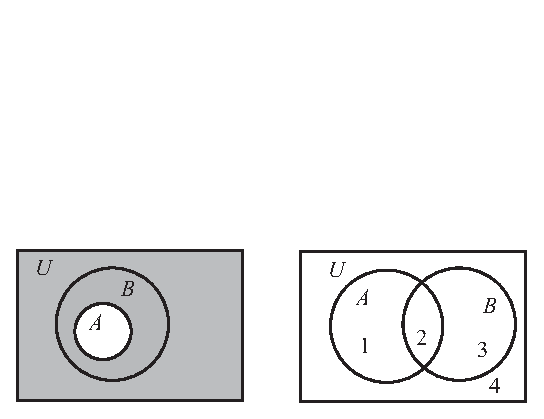
\includegraphics{figps-prev52.eps}
\caption{Venn Diagrams for Beginning Activity 2} \notag
\end{center}
\end{figure}

\hbreak

\end{document}

\begin{center}
\begin{table}[h!]
\begin{tabular}[h!]{|p{0.4in}|p{2in}|p{1.8in}|}
  \hline
  \textbf{Step}  &  \textbf{Know}  &  \textbf{Reason}     \\ \hline
  $P$     &  $S$  is the set of all integers that are multiples of 6.
$T$ is the set of all even integers.
     &  Hypothesis \\ \hline
  $P1$    &   Let  $x \in S$.        &  Choose an arbitrary element of  $S$.     \\ \hline
  $P2$  &  $\left( {\exists m \in \mathbb{Z}} \right)\left( {x = 6m} \right)$  &  Definition of ``multiple''  \\  \hline
  $P3$  &  $x = (2 \cdot 3 ) m$        & $6 = 2 \cdot 3$ \\ \hline
  $P4$  &  $x = 2 (3m)$                &  Associative Law \\ \hline
  $P5$  &  $x$ is even.                &  Definition of an even integer since $3m$ is an integer. \\ \hline
  $Q2$   &  $x$   is an element of  $T$.  &  $x$ is even.  \\  \hline
  $Q1$    &   $\left( \forall x \in \Z \right) \left[ \left( x \in S \right) \to \left( x \in T \right) \right]$                         & Step  $P1$  and Step $Q2$            \\  \hline  
  $Q$     &  $S \subseteq T$                     &  Definition of ``subset''     \\ \hline
  \textbf{Step}  &  \textbf{Show}  &  \textbf{Reason}     \\ \hline
\end{tabular}
\end{table}
\end{center}
